\hypertarget{group__Launcher}{\section{Launcher}
\label{group__Launcher}\index{Launcher@{Launcher}}
}


Tools for launching H\-P\-C jobs.  


Collaboration diagram for Launcher\-:
\nopagebreak
\begin{figure}[H]
\begin{center}
\leavevmode
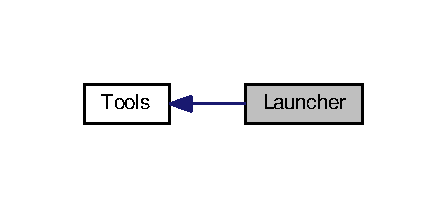
\includegraphics[width=214pt]{group__Launcher}
\end{center}
\end{figure}
Tools for launching H\-P\-C jobs. \hypertarget{group__Launcher_ALPS}{}\subsection{A\-L\-P\-S}\label{group__Launcher_ALPS}

\begin{DoxyParams}{Parameters}
{\em hostfile} & The hostfile for \hyperlink{namespaceOpenMPI}{Open\-M\-P\-I} to use \\
\hline
{\em command} & Command for executing the application \\
\hline
{\em np} & Number of processes to run \\
\hline
{\em options} & Comma-\/delimited sets of command line options that shall be used on each test \\
\hline
{\em skipped} & Exit status of a test that declares it was skipped \\
\hline
{\em merge\-\_\-stdout\-\_\-stderr} & Merge stdout and stderr into one output stream \\
\hline
{\em stdout\-\_\-save\-\_\-lines} & Number of lines of stdout to save \\
\hline
{\em stderr\-\_\-save\-\_\-lines} & Number of lines of stderr to save \\
\hline
{\em test\-\_\-dir} & Names of directories to be scanned for tests \\
\hline
{\em fail\-\_\-tests} & Names of tests that are expected to fail \\
\hline
{\em fail\-\_\-returncodes} & Expected returncodes of tests expected to fail \\
\hline
{\em fail\-\_\-timeout} & Maximum execution time for tests expected to fail \\
\hline
{\em skip\-\_\-tests} & Names of tests to be skipped \\
\hline
{\em max\-\_\-num\-\_\-tests} & Maximum number of tests to run \\
\hline
{\em modules} & Modules to load \\
\hline
{\em modules\-\_\-unload} & Modules to unload \\
\hline
{\em test\-\_\-list} & List of tests to run, default is all \\
\hline
{\em allocate\-\_\-cmd} & Command to use for allocating nodes from the resource manager \\
\hline
{\em deallocate\-\_\-cmd} & Command to use for deallocating nodes from the resource manager\\
\hline
\end{DoxyParams}
\hypertarget{group__Launcher_OpenMPI}{}\subsection{Open\-M\-P\-I}\label{group__Launcher_OpenMPI}

\begin{DoxyParams}{Parameters}
{\em hostfile} & The hostfile for \hyperlink{namespaceOpenMPI}{Open\-M\-P\-I} to use \\
\hline
{\em command} & Command for executing the application \\
\hline
{\em np} & Number of processes to run \\
\hline
{\em ppn} & Number of processes per node to run \\
\hline
{\em timeout} & Maximum execution time -\/ terminate a test if it exceeds this time \\
\hline
{\em options} & Comma-\/delimited sets of command line options that shall be used on each test \\
\hline
{\em skipped} & Exit status of a test that declares it was skipped \\
\hline
{\em merge\-\_\-stdout\-\_\-stderr} & Merge stdout and stderr into one output stream \\
\hline
{\em stdout\-\_\-save\-\_\-lines} & Number of lines of stdout to save \\
\hline
{\em stderr\-\_\-save\-\_\-lines} & Number of lines of stderr to save \\
\hline
{\em test\-\_\-dir} & Names of directories to be scanned for tests \\
\hline
{\em fail\-\_\-tests} & Names of tests that are expected to fail \\
\hline
{\em fail\-\_\-returncodes} & Expected return codes of tests expected to fail \\
\hline
{\em fail\-\_\-timeout} & Maximum execution time for tests expected to fail \\
\hline
{\em skip\-\_\-tests} & Names of tests to be skipped \\
\hline
{\em max\-\_\-num\-\_\-tests} & Maximum number of tests to run \\
\hline
{\em test\-\_\-list} & List of tests to run, default is all \\
\hline
{\em allocate\-\_\-cmd} & Command to use for allocating nodes from the resource manager \\
\hline
{\em deallocate\-\_\-cmd} & Command to use for deallocating nodes from the resource manager\\
\hline
\end{DoxyParams}
\hypertarget{group__Launcher_SLURM}{}\subsection{S\-L\-U\-R\-M}\label{group__Launcher_SLURM}

\begin{DoxyParams}{Parameters}
{\em hostfile} & The hostfile for \hyperlink{namespaceOpenMPI}{Open\-M\-P\-I} to use \\
\hline
{\em command} & Command for executing the application \\
\hline
{\em np} & Number of processes to run \\
\hline
{\em timeout} & Maximum execution time -\/ terminate a test if it exceeds this time \\
\hline
{\em options} & Comma-\/delimited sets of command line options that shall be used on each test \\
\hline
{\em skipped} & Exit status of a test that declares it was skipped \\
\hline
{\em merge\-\_\-stdout\-\_\-stderr} & Merge stdout and stderr into one output stream \\
\hline
{\em stdout\-\_\-save\-\_\-lines} & Number of lines of stdout to save \\
\hline
{\em stderr\-\_\-save\-\_\-lines} & Number of lines of stderr to save \\
\hline
{\em test\-\_\-dir} & Names of directories to be scanned for tests \\
\hline
{\em fail\-\_\-tests} & Names of tests that are expected to fail \\
\hline
{\em fail\-\_\-returncodes} & Expected returncodes of tests expected to fail \\
\hline
{\em fail\-\_\-timeout} & Maximum execution time for tests expected to fail \\
\hline
{\em skip\-\_\-tests} & Names of tests to be skipped \\
\hline
{\em max\-\_\-num\-\_\-tests} & Maximum number of tests to run \\
\hline
{\em job\-\_\-name} & User-\/defined name for job \\
\hline
{\em modules} & Modules to load \\
\hline
{\em modules\-\_\-unload} & Modules to unload \\
\hline
{\em test\-\_\-list} & List of tests to run, default is all \\
\hline
{\em allocate\-\_\-cmd} & Command to use for allocating nodes from the resource manager \\
\hline
{\em deallocate\-\_\-cmd} & Command to use for deallocating nodes from the resource manager \\
\hline
\end{DoxyParams}
